\documentclass[a4paper, 11pt]{article}
\usepackage[english]{babel}
\usepackage{amsthm, amsmath, amssymb}
\usepackage{graphicx}% includegraphics
\usepackage{array}   % outline of p{} elements in tables
\usepackage{enumitem}% control spacing in lists
\usepackage{caption} % for non-floating tables
\usepackage{listings}

\lstset{numbers=left,
language=C
}

\usepackage[
  pdfborder={0,0,0},
  colorlinks=true,
  linkcolor=black,
  citecolor=black,
  urlcolor=blue
]{hyperref}
\usepackage{natbib}
\bibliographystyle{chicago}

\newtheorem{demand}{Demand}
\newtheorem{definition}{Definition}



\renewcommand{\familydefault}{\sfdefault}

\newcommand{\code}[1]{\texttt{#1}}
\newcommand{\waar}{{\normalfont \texttt{True}}}
\newcommand{\onwaar}{{\normalfont \texttt{False}}}
\newcommand{\na}{{\normalfont \texttt{NA}}}

\newcommand{\la}[1]{\boldsymbol{#1}}

\title{Validation report structure}
\author{Mark van der Loo and Olav ten Bosch}
\date{\today}




\setlength{\parindent}{0pt}
\setlength{\parskip}{2ex}

\begin{document}

\maketitle{}

\tableofcontents{}


\section{Introduction}

\section{Demands on a validation report}
Figure~\ref{fig:validation} gives a high-level overview of a data validation
procedure. At the input side, we find the data to be validated and the
validation rules that the data are supposed to satisfy. At some point in time,
the data are confronted with the rules and validation results are created. 
%
\begin{figure}[t]
\centering
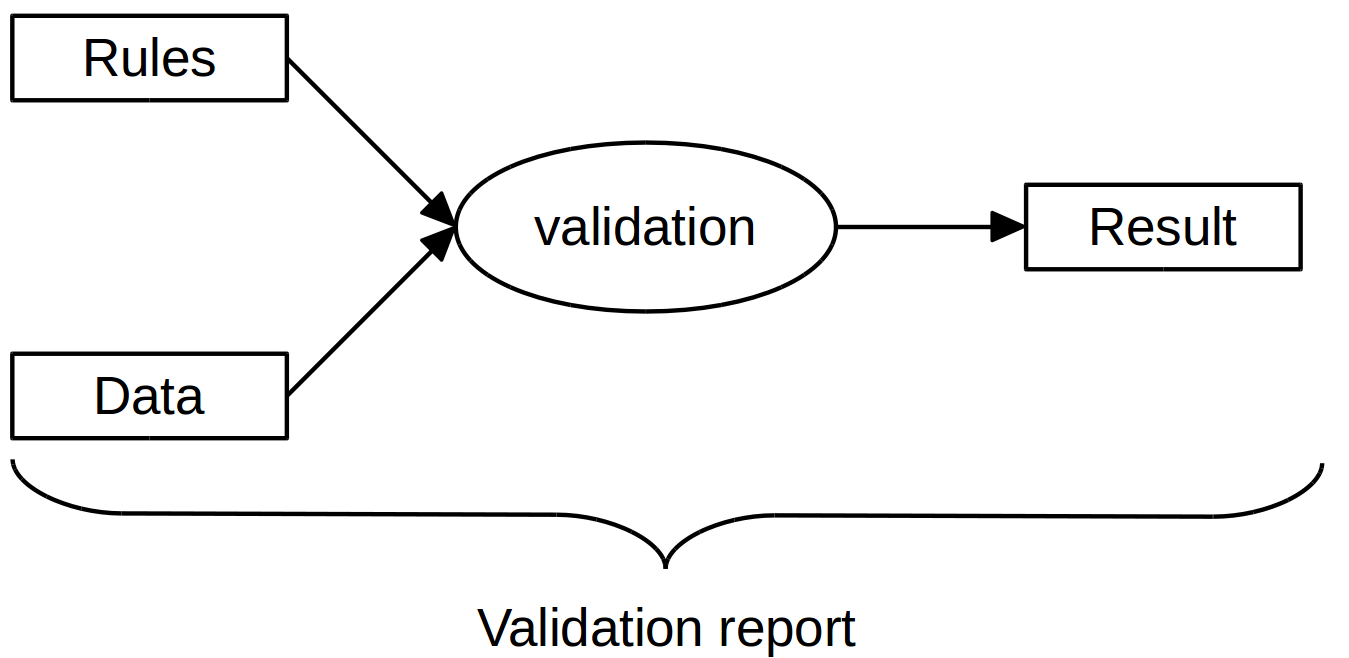
\includegraphics[width=0.7\textwidth]{fig/validation.png}
\caption{Information elements involved in creating a validation result, relevant for validation reports.}
\label{fig:validation}
\end{figure}

The purpose of a validation report is to convey validation results and
information on the validation procedure. The procedure as a whole generates and
processes a lot of information that can possibly be included in such a report.
For example, the validation rules may be endowed with metadata such as
descriptions and severity level and for the validation procedure it may be
interesting to record a timestamp and the used software.

A relevant question to ask is therefore what information should be included in
a validation report. Conceptually we can explore the extreme possibilities on a
scale such as depicted in Figure~\ref{fig:richness}. On the left, we find a minimal report
containing a single result only: True, meaning that all data passed all rules,
or False, meaning that not all data passed all rules. On the right extreme, the
report conveys all data and metadata associated with the validated data, the
validation rules, the validation procedure and the results.
%
\begin{figure}
\centering
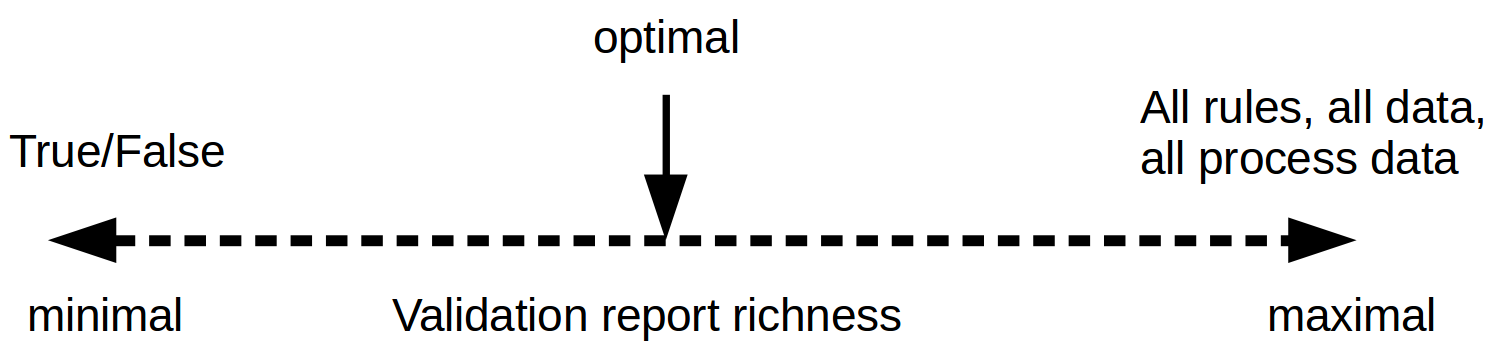
\includegraphics[width=0.8\textwidth]{fig/richness.png}
\caption{Possible content of validation reports on a conceptual scale of 'richness'.}
\label{fig:richness}
\end{figure}


Before moving to a formal discussion of the information items involved with
data validation, it is useful to discuss a number of demands on a validation
report that will serve all uses and users. First of all, we take as a given
that a result that cannot be identified with the data and rules it pertains to
is useless. If the reports are to be used for communication accross
organizations, or if they are to interpreted separately from the process that
triggered the validation, the relation with the rules and data needs to be
included.  In fact, this can also be seen as a direct consequence of the
validation principle \emph{Well-documented and appropriately communicated
validation errors} \citep{ESS2017}. This leads us to the following demand.

\begin{demand}[Identification]
A validation report shall convey validation results such that they can be
identified with the validation procedure, the validation rules used, and the
validated data.
\label{dem:identify}
\end{demand}


A validation procedure usually involves multiple rules and each rule may
pertain to different subsets of variables, records or reference datasets. Every
confrontation of a rule with the data can be seen as a validation
(sub)procedure yielding a validation report. To gather all results, validation
reports should be able to be combined to an overall report.
%
\begin{demand}[Closure under combination]
Two validation reports shall be combinable in such a way that the result is
again a validation report that includes all information that separate reports
contained.
\label{dem:combine}
\end{demand}
%
This includes cases where multiple procedures are involved, possibly pertaining
to varying datasets, rulesets and actors involved in the validation procedures. 

Finally, depending on intended use, one may be interested in the details of
each step in each validation procedure, or in a more aggregated view of one or
more validation events. Indeed, a quick view on some example validation reports
from multiple NSI's and multiple statistical domains shows that most of them
contain some kind of aggregated results within the validation report itself.
Therefore, we also demand the following.

\begin{demand}[Closure under aggregation]
A validation report can be aggregated such that the result is again a
validation report.
\label{dem:aggregate}
\end{demand}

Here, many types of aggregation may be relevant, including counting the
(relative) number of passes and fails, finding the procedure that yielded the
maximum number of fails (or passes), and so on.

Both the second and third demand mention the term \emph{closure} which may not be a
familiar term to all readers. The term `closure' or `algebraic closure' refers
to the property of a set being invariant under certain operations. For example,
since the sum of any two natural numbers is again a natural number, we can say
that ‘the natural numbers are closed under addition’. For our purposes it is
important that the result of combining or aggregating a validation report is
also a validation report, meaning that it has exactly the same structure (but
possibly different content) before or after aggregation. If this is not the
case, we run the risk of defining new data structures for each aggregate or
combination of reports.

As it turns out, adding both closure under combination and closure under
aggregation to the demand of identifiability significantly increases the
complexity of the structure of a validation report. Since aggregates can always
be derived from a set of `atomic' validation results, we therefore propose two
types of interchange formats. The first is called the \emph{basic validation
report structure} and it conveys the rule-by-rule and event-by-event validation
results, dropping Demand~\ref{dem:aggregate}. It is a simple format that is
representable as a rectangular data structure from which (possibly
grouped) aggregations can easily be computed.  The second is called
\emph{extended validation report structure}. This structure is richer and
allows for precomputed aggregates.  Since aggregation endows a graphical
structure on a record, parsing such a structure is more involved.



%%%%%%%%%%%%%%%%%%%%%%%%%%%%%%%%%%%%%%%%%%%%%%%%%%%%%%%%%%%%%%%%%%%%%%%%%%%%%%%
\section{Identifying validation results}
To get an idea of the (meta)data necessary to identify a validation result,
consider the data, validation rules and validation results shown in
Table~\ref{tab:example1}. When a dataset is confronted with a validation rule,
there are three possible outcomes. A rule can be satisfied, yielding \waar{}, a
rule can be failed, yielding \onwaar{}, or a rule cannot be evaluated because
of missing data, yielding \na{}.
%
\begin{table}
\centering
\caption{Example data, validation rules, and results}
\begin{tabular}{rccccb{4cm}}
\hline
&\multicolumn{2}{c}{\textbf{Variables}}&&\multicolumn{2}{c}{\textbf{Rules}}\\
Nr  & Age  & hasjob     && \code{Age >= 0} & \code{IF Age < 15 THEN hasjob == `no'}\\
\cline{2-3}\cline{5-6}
1   & 36   & \code{yes} && \waar{}        & \multicolumn{1}{c}{\waar{}}\\
2   & 53   & \code{NA}  && \waar{}        & \multicolumn{1}{c}{\na{}}\\
3   & 11   & \code{yes} && \waar{}        & \multicolumn{1}{c}{\onwaar{}}\\
\hline
\end{tabular}
\label{tab:example1}
\end{table}



In the example three records on age and work status are checked against two
rules: age must be larger than or equal to zero, and persons under 15 years old
cannot have a job. In each case the demand on  age can be checked and and each
record passes this test, yielding \waar{} as validation result. For the second
rule, the first record passes the check since age equals 36 and the person has
a job which is allowed by the rule. In the second case the job status is not
available (\na{}). Hence the rule cannot be checked and the returned value is \na{}
as well. Finally, in the third record there is an 11-year old with a job which
is a combination that is not allowed by the rule, yielding \onwaar{}.


The above discussion leads to the following definition of a validation result.
%
\begin{definition}[Validation result]
A validation result is a value from the set $\{\waar{},\onwaar{},\na{}\}$.
\label{def:validationresult}
\end{definition}
Validation results are obtained as outcomes of evaluating a validation rule on
a data set.

A recurring point of discussion is whether \na{} should be an allowed
validation result. The main other options are to either interrupt execution, or
to interpret the result as failed (\onwaar{}) when one of the data points
necessary for evaluating a rule is missing. Because statistical data often
suffers from missing data the first option would yield many interruptions of a
statistical process flow, unless each rule guards against it by building in
clauses that detect missing values explicitly. The second option (\na{} implies
\onwaar{}) would yield a loss of information. More importantly, it assumes
(possibly unwarranted) that the user of the result follows this interpretation.

We deem both alternatives undesirable and therefore follow the definition
above, which also agrees with the definition of a formal data validation
function in the Methodology on Validation handbook published by the Validat
Foundation \cite{zio2015methodology}.

\subsection{Validation events}

With a \emph{validation event} we mean the physical activity where a dataset is
confronted with a single rule, yielding precisely one validation result. A
validation event is characterized by its inputs (the rule and the dataset it
pertains to) as well as its own metadata, including the time of execution and
the actor performing the execution. We therefore adopt the following convention
by defining a set of keys that identifies such a physical event.
%
\begin{definition}[validation event] 
A validation event is a triple $(e,r,d)$, where $e$ identifies metadata of the
physical event, $r$ identifies the evaluated validation rule and $d$ identifies
the data points involved in the evaluation.
\label{def:validaitonevent}
\end{definition}
%
We leave open the possibility that each component $e$, $r$ and $d$ consists of
informative tuples to identify subcomponents of the event, data or rule.  Note
that the above `definition' is not a definition in the mathematical sense.
Rather it is a convention that can be tested in a (software) environment where
data, rules, and validation events have been labeled and stored.

 
\section{Basic validation reports}
The concepts of a validation result and a validation event now allow us to 
give a recursive definition of a validation report.
%
\begin{definition}[Basic validation report]\leavevmode
\begin{enumerate}[topsep=0pt,itemsep=0pt]
\item The empty set $\{\}$ is a basic validation report.
\item If $\la{k}$ is a validation event and $v$ its validation result, then $\{(\la{k},v)\}$
is a basic validation report.
\item If $V$ and $W$ are basic validation reports, then the set union $V\cup
W$, set difference $V-W$ and set intersection $V\cap W$ are validation reports.
\end{enumerate}
\end{definition}
%
It follows trivially that any subset of a basic validation report is a
basic validation report. The event key $\la{k}$ ensures identifiability of the
validation result $v$ for each element of a report (Demand~\ref{dem:identify}),
while the set union ensures that reports can be combined
(Demand~\ref{dem:combine}).


\subsection{Structure of a basic validation report}
Below, we detail the minimum information to include in each slot of a formal 
validation event. Every table has four columns, with the following contents.
\begin{enumerate}
\item Item: the name of the slot.
\item Format: technical format of the data in the slot. Allowed formats are: \code{string},
\code{numeric}, \code{enum} (with categories defined in the description column), \code{datetime} and
\code{-}. The latter indicates that the format is free, including the possibility to include user-defined objects.
\item Description: a short description of the slot. More detailed descriptions
might follow after the table.
\item Example: an example.
\end{enumerate}
%
The information in these Tables is mandatory. For each table it is also
indicated whether it is allowed to extend it with user-defined information.


The different data types are to be formatted according to commonly used
standards where possible. In particular, data in validation reports shall be
encoded as stated in Table~\ref{tab:dataformat}.
\begin{center}
\captionof{table}{Format of data types in validation reports (basic or extended).}
\begin{tabular}{|lp{0.92\textwidth}|}
\hline
1&Numbers shall be encoded in a valid decimal ISO/IEC/IEEE 60559:2011 (IEEE 754) format \\
2&Date-time data shall be denoted in ISO 8601 format \code{YYMMDDTHHmmss+HHMM}. \\
3&Enumerated data types are encoded as a string from the set predefined in the item's description.\\
\hline
\end{tabular}
\label{tab:dataformat}
\end{center}

The following Tables fix the information content of each item making up elements of 
a validation report: $e$, $r$, $d$, and $v$.

%%%%%%%%%%%%%%%%%%%%%%%%%%%%%%%%%%%%%%%%%%%%%%%%%%%%%%%%%%%%%%%%%%%%%%%%%%%%%%%
\subsubsection{Identification of a physical validation event.}
%
\begin{center}
\captionof{table}{Mandatory identification of a physical validation event $e$.}
\begin{tabular}{|lp{15mm}p{0.34\textwidth}p{0.34\textwidth}|}
\hline
\textbf{Item} & \textbf{Format} & \textbf{Description} &\textbf{Example}\\
\hline
time          & datetime & Time marking the completion of a validation event. & \code{20170212T101530+0100}\\
actor         & string        a  & Software that or person who created the validation result. & \code{R package validate version 0.1.7}\\
\hline
\multicolumn{4}{|l|}{The number of slots defining a validation event is \textbf{extendable}.
}\\
\hline
\end{tabular}
\end{center}


\begin{center}
\captionof{table}{Recommended information on a physical validation event $e$.}
\begin{tabular}{|lp{15mm}p{0.34\textwidth}p{0.34\textwidth}|}
\hline
\textbf{Item} & \textbf{Format} & \textbf{Description} &\textbf{Example}\\
\hline
agent   & \multicolumn{1}{c}{-} & Actor (person, institute, dpt) responsible for executing the validation event & dpt. of data validation, Eurostat\\
trigger & \multicolumn{1}{c}{-} & Actor (person, institute, dpt) responsible for triggering the event  & John Statistician, Statistics Netherlands\\
\hline
\end{tabular}
\label{tab:recommendedevent}.
\end{center}
The recommended slots of Table~\ref{tab:recommendedevent} are useful, especially when validation is executed as a (remote) service.


%%%%%%%%%%%%%%%%%%%%%%%%%%%%%%%%%%%%%%%%%%%%%%%%%%%%%%%%%%%%%%%%%%%%%%%%%%%%%%%
\subsubsection{Identification of a validation rule}
%
\begin{center}
\captionof{table}{Mandatory identification of validation rule $r$.}
\begin{tabular}{|lp{15mm}p{0.34\textwidth}p{0.34\textwidth}|}
\hline
\textbf{Item} & \textbf{Format} & \textbf{Description} &\textbf{Example}\\
language      & string   & Language and version in which a rule is expressed & R/validate version 0.1.7\\
expression    & string   & Expression defining the rule           & \code{age >= 0}\\
severity      & enum     & \code{`error'}, \code{`warning'},
                           or \code{`information'}                & \code{`information'}\\ 

\hline
\multicolumn{4}{|l|}{The number of slots defining a validation rule is \textbf{extendable}.
}\\
\hline
\end{tabular}
\end{center}


%%%%%%%%%%%%%%%%%%%%%%%%%%%%%%%%%%%%%%%%%%%%%%%%%%%%%%%%%%%%%%%%%%%%%%%%%%%%%%%
\subsubsection{Identification of the validated data}
Although generic models for identifying a data point exist [e.g.
\citet[Chapter~5]{zio2015methodology}], it will in practice often depend on the
local implementation of a local data model. Therefore, little limits are posed
on the keys involved in pointing out the data used in an evaluation. However,
as a general rule, it should be clear 
\begin{itemize}[itemsep=0pt]
\item to which population the data under scrutiny pertains;
\item the identity of the process that yielded the data (`time of measurement');
\item to which units in the population the data pertains;
\item what variables are measured by the data.
\end{itemize}
These are the four components defined in the Methodology of validation handbook 
\citep{zio2015methodology}.


\begin{center}
\captionof{table}{Mandatory identification of validated data $d$.}
\begin{tabular}{|lp{15mm}p{0.34\textwidth}p{0.34\textwidth}|}
\hline
\textbf{Item} & \textbf{Format} & \textbf{Description} &\textbf{Example}\\
data    &\multicolumn{1}{c}{-} & A set of key(s) or other identification (e.g.
a query statement) identifying the data used in evaluating the validation rule
&  (`people in NL', `SILC2016, `Ria Respondent', `Income')\\
\hline
\multicolumn{4}{|l|}{The number of slots defining a validation rule is \textbf{extendable}.
}\\
\hline
\end{tabular}
\end{center}


Allowing for implicit definition of the (sub)set of data touched by a
validation rule potentially reduces the size of a validation report
significantly: it is possible to have millions of datapoints involved in a
single validation rule. The trade-off is that aggregating validation reports,
grouped by properties of the data directly is not possible.

\begin{tabular}{|p{0.97\textwidth}|}
\hline
It is recommended that for validation rules that can be evaluated using a
single datapoint only (e.g. \code{income >= 0}), the data is identified using a
key (or array of keys) directly related to the data value under scrutiny.\\
\hline
\end{tabular}

\subsubsection{Validation result}

\begin{center}
\captionof{table}{Mandatory format for the validation result $v$.}
\begin{tabular}{|lp{15mm}p{0.34\textwidth}p{0.34\textwidth}|}
\hline
\textbf{Item} & \textbf{Format} & \textbf{Description} &\textbf{Example}\\
value  & \code{enum} & \waar{}, \onwaar{}, or \na{}    &\waar{}\\
\hline
\multicolumn{4}{|l|}{The number of slots defining a validation result \textbf{not extendable}.
}\\
\hline
\end{tabular}
\end{center}

\subsection{JSON schema for basic validation reports}
The code on Page~\pageref{code:basicreport} shows a JSON schema implementing
a format for storing and transmitting the information items described in the previous
paragraphs. 

\newpage
\label{code:basicreport}
\lstinputlisting[frame=single]{../json/basic_validation_report.json}


\section{Extended validation report structure}



\bibliography{report}

\end{document}
